\documentclass[DIV=calc, paper=a4, fontsize=11pt, twocolumn]{scrartcl}
\usepackage{microMathematics-br}
\usepackage[portuguese]{babel} % Rortuguese language/hyphenation

% Begin document
\begin{document}
\maketitle
\thispagestyle{fancy} % Enabling the custom headers/footers for the first page

\begin{bf}
% This is the first part of the file about_micromath.tex
El microMathematics Plus es la
calculadora matemática en Android
orientada alrededor de una hoja de cálculo que
permite la edición en vivo de identidades matemáticas
combinadas con cálculos altamente
precisos.

Basada en una potente pantalla táctil
el editor permite a los usuarios crear y
manipular de forma natural
hojas de trabajo que contienen todas las
anotaciones matemáticas básicas.

El microMathematics Plus permite
operar matemáticas al nivel de educación
secundaria. Esta versión tiene
siguientes limitaciones matemáticas: no soporta funciones especiales,
vectores, matrices y muchas otras
cosas de matemáticas de alto nivel.
\end{bf}

\section{Utilizar}
% This is auto-generated file: do not edit!
% Exported from microMathematics Plus, version 2.18.0


Este app é um poderoso programa
calculador em formato de folha de
cálculos. A folha de cálculos pode ser
editada livremente, armazenada no
cartão SD, aberta de um cartão SD e
exportada para uma imagem ou formato
LaTeX.

A folha de cálculos é um documento
matemático que contém texto, fórmulas
e gráficos. Ela suporta edição em
tempo real de notações matemáticas e
seu cálculo automático.

Os objetos a seguir podem ser
inseridos na folha de cálculos:
equações, janelas de resultado,
gráficos, fragmentos de textos e
imagens. Este documento fornece uma
visão geral de como editar estes
objetos.

\subsection{Edição}

Quase todos os objetos disponíveis
possuem vários campos editáveis. Para
editar o campo use os símbolos e
funções na barra de ferramentas.

Todos os símbolos podem ser entrados
pelo teclado. Para encontrar qual
símbolo do teclado corresponde ao
símbolo matemático que você deseja,
leia a dica segurando o botão de
interesse.

Ao segurar em um termo você pode
selecionar este termo. O termo
selecionado pode ser excluído, copiado
para a área de transferência, colado
da área de transferência ou outra
operação ou função pode ser inserida
depois do termo usando os botões da
barra de ferramentas ou teclado.

O comando ''Desfazer'' está disponível
na barra de ações. Ele apaga a última
mudança feita ao documento e reverte-a
para um estado anterior:
\begin{center}\begin{tabular}{c} 
\includegraphics[resolution=320]{graphics/how_to_use_fig1.png} \end{tabular}\end{center}

\subsection{Equação}

Uma equação define uma constante
numérica, um intervalo ou uma função.
Para criar uma equação, use o botão
''Novo elemento'' na barra de ações
\begin{center}\begin{tabular}{c} 
\includegraphics[resolution=320]{graphics/how_to_use_fig2.png} \end{tabular}\end{center}

ou o botão ''Adicionar equação'' da barra
de ferramentas:
\begin{center}\begin{tabular}{c} 
\includegraphics[resolution=320]{graphics/how_to_use_fig3.png} \end{tabular}\end{center}

Uma equação com dois campos vazios
aparece. Estes campos devem ser
preenchidos:
\begin{center}\begin{tabular}{c}
  ${\Box} := {\Box}$
\end{tabular}\end{center}

O nome da equação é dado no campo
esquerdo. O nome deve conter letras ou
dígiros apenas e srá usado em outros
objetos para referenciar esta equação.

A partir da barra de ações, você pode
abrir a janela de ''Configurações do
documento'': 
\begin{center}\begin{tabular}{c} 
\includegraphics[resolution=320]{graphics/how_to_use_fig4.png} \end{tabular}\end{center}

Dependendo do parâmetro ''Permitir
re-definir equações'' nesta janela, há
dois modos de uso:

a) se a redefinição não for permitida,
o nome da equação deve ser único
dentro de todo o espaço de trabalho e
a equação pode ser usada antes e
depois de ser definida,

b) se a redefinição for permitida,
você pode redefinir mais de uma
equação com o mesmo nome. Se esta
equação está referenciada, a última
versão definida antes de chamar a
função será usada.

\subsubsection{Constante}

Se o nome da equação não contém nenhum
argumento entre parênteses, isso
define uma constante ou um intervalo:
\begin{center}\begin{tabular}{ccc}
  $N := 200$ &
  $Sq2 := \sqrt{100} $ &
  $Pi2 := \frac{{\pi}}{2}$ \cr
\end{tabular}\end{center}

Neste último exemplo, uma constante
embutida pi foi usada. Atualmente, as
seguintes constantes embutidas estão
disponíveis:
\begin{center}\begin{tabular}{ccc}
  ${\pi} = 3.14159$ &
  $pi = 3.14159$ &
  $e = 2.71828$ \cr
\end{tabular}\end{center}

Uma constante definida anteriormente
também pode ser usada:
\begin{center}\begin{tabular}{c}
  $NPi2 := N \cdot Pi2$
\end{tabular}\end{center}

Você também pode usar o símbolo ''i''
como unidade imaginária para poder
definir um número complexo:
\begin{center}\begin{tabular}{c}
  $z := 5+3i$
\end{tabular}\end{center}

\subsubsection{Intervalo}

Uma equação do tipo intevalo define uma
variável qur foi alterada de um valor
minímo dado até um valor máximo dado
com incremento definido. Esta variável
pode ser usada como o argumento do
gráfico de uma função ou como um
parâmetro para construir uma tabela de
valores da função.

Para definir um intervalo, insira um
nome válido no lado esquerdo de uma
equação vazia. No lado direito desta
equação, coloque um símbolo '':'', ou
toque no botão ''Intervalo
equidistante'' da barra de ferramentas:
\begin{center}\begin{tabular}{c} 
\includegraphics[resolution=320]{graphics/how_to_use_fig5.png} \end{tabular}\end{center}

Aqui, o primeiro elemento é o ponto
inicial do intervalo, o próximo
elemento é o segundo ponto, e o último
elemento é o ponto final do intervalo:
\begin{center}\begin{tabular}{c}
  $x := \left[ 0,\, 0.1 \,..\, 10 \right]$
\end{tabular}\end{center}

Os elementos do intervalo podem ser
acessados como segue:
\begin{center}\begin{tabular}{ccc}
  $x_{0}  = 0.0$ &
  $x_{1}  = 0.1$ &
  $x_{100}  = 10.0$ \cr
\end{tabular}\end{center}

O incremento é a diferença entre o
segundo e o primeiro valores:
\begin{center}\begin{tabular}{c}
  $x_{2}  - x_{1}  = 0.1$
\end{tabular}\end{center}

Por exemplo, podemos definir um
intervalo equidistante que contém N
pontos distribuídos com incremento
''dy'' onde o início do intervalo é zero
como segue:
\begin{center}\begin{tabular}{cc}
  $dy := 0.05$ &
  $y := \left[ 0,\, dy \,..\, dy \cdot N \right]$ \cr
\end{tabular}\end{center}

\subsubsection{Function}

Uma função é uma relação entre um ou
mais argumentos e um conjunto de
saídas permissivas com a propriedade,
que cada valor do argumento (real ou
complexo) ou a combinação de
argumentos está relacionada à
exatamente uma saída.

O nome da função e o argumento entre
parênteses são dados no lado esquerdo
da equação. Não é necessário definir o
argumento na folha de trabalho
anteriormente, você pode definí-lo
como quiser, mas usando apenas letras
ou dígitos:
\begin{center}\begin{tabular}{c}
  $f(t) := sin \left( t\right)  \cdot cos \left( t\right)  / 2$
\end{tabular}\end{center}
\begin{center}\begin{tabular}{c}
  $w(z) := {e}^{2i \cdot {\pi} \cdot z}$
\end{tabular}\end{center}
\begin{center}\begin{tabular}{c}
  $H(x,y) := \sqrt{{x}^{2} + {y}^{2}} $
\end{tabular}\end{center}
\begin{center}\begin{tabular}{c}
  $g(x,y) := \frac{sin \left( H \left( x,\, y\right) \right) }{H \left( x,\, y / 2\right)  + 1}$
\end{tabular}\end{center}

O lado direito da função contém uma
fórmula matemática de como calcular a
função. Se esta fórmula não contém o
argumento da função declarado, tal
função será interpretada como uma
constante.

Você também pode usar o lado direito
ou outras funções embutidas ou
previamente definidas. Para inserir um
função entre o nome dela, toque no
abre parênteses
 ''('' e então entre o argumento. Este
argumento também pode ser uma fórmula,
que contém quaisquer outras operações
e funções.

\subsubsection{Array}

Arranjos são funções especiais com as
seguintes propriedades:

a) apenas um intervalo previamente
definido pode ser usado como um
argumento de arranjo:
\begin{center}\begin{tabular}{cc}
  $k := \left[ 0,\, 1 \,..\, 100 \right]$ &
  $m := \left[ 0,\, 1 \,..\, 200 \right]$ \cr
\end{tabular}\end{center}

a) argumentos de arranjos são dados
entre [ ] ao invés de ( ):
\begin{center}\begin{tabular}{c}
  $M[k,m] := {sin \left( k / 10\right) }^{2} - 3 \cdot  \left| cos \left( m / 10\right)  \right| $
\end{tabular}\end{center}

c) elementos de arranjos são calculados
e armazenados na memória que reduz o
tempo de acesso à esses valores

d) elementos de arranjos podem ser
acessados apenas usando um índice
menor. Para criar um índice menor,
coloque ''['' após o nome do arranjo:
\begin{center}\begin{tabular}{cc}
  $M_{5,\, 10}  = -1.39106$ &
  $M_{10,\, 5}  = -1.92467$ \cr
\end{tabular}\end{center}
\begin{center}\begin{tabular}{c}
  $P[k,m] := floor \left( -10 \cdot M_{k,\, m} \right) $
\end{tabular}\end{center}

e) se qualquer índice do arranjo for
complexo ou negativo ou maior que o
limite superior do intervalo
correspondente, o número inválido será
retornado:
\begin{center}\begin{tabular}{cc}
  $M_{10i,\, 100}  = NaN$ &
  $M_{90,\, 210}  = NaN$ \cr
\end{tabular}\end{center}

\subsection{Result View}

Este elemento é usado para representar
um resultado de cálculo como um número
ou uma tabela. Para adicionar este
elemento, use o botão ''Novo elemento''
na barra de ações ou o botão
''Adicionar janela de resultado'' da
barra de ferramentas:
\begin{center}\begin{tabular}{c} 
\includegraphics[resolution=320]{graphics/how_to_use_fig6.png} \end{tabular}\end{center}

Uma equação com dois campos aparece,
onde o campo esquerdo deve ser
preenchido:
\begin{center}\begin{tabular}{c}
  ${\Box} = {\Box}$
\end{tabular}\end{center}

O termo da esquerda contém uma fórmula
para ser calculada e o termo da
direita é o resultado do cálculo. O
resultado será mostrado quando você
pressionar o botão flutuante
''Calcular''.

No termo da esquerda você pode usar
quaisquer constantes e funções
definidas previamente assim como
quaisquer funções embutidas:
\begin{center}\begin{tabular}{c}
  ${e}^{{\pi}} \cdot f \left( NPi2\right)  = 2.27286E-14$
\end{tabular}\end{center}

Se a parte da esquerda não contém
nenhuma variável ''parecida com
intervalo'', o resultado do cálculo é
apenas um número real ou complexo:
\begin{center}\begin{tabular}{c}
  $y_{N - 1}  - y_{0}  = 9.95$
\end{tabular}\end{center}
\begin{center}\begin{tabular}{ccc}
  $\Re\left( z \right)  = 5.0$ &
  $\Im\left( z \right)  = 3.0$ &
  $ \left| z \right|  = 5.83095$ \cr
\end{tabular}\end{center}
\begin{center}\begin{tabular}{c}
  $\sqrt{sin \left( \frac{3}{2} \cdot {\pi}\right) }  = 0.0+1.0i$
\end{tabular}\end{center}

Se a parte da esquerda contém uma
variável de intervalo, o resultado do
cálculo será um vetor de valores
correspondentes à este intervalo.
Devido ao limite de espaço livre na
tela, apenas os primeiros e últimos
elementos do vetor serão exibidos:
\begin{center}\begin{tabular}{ccc}
  $x = \begin{bmatrix}0.0\\0.1\\0.2\\0.3\\0.4\\0.5\\\dots\\10.0\\\end{bmatrix}$ &
  $y = \begin{bmatrix}0.0\\0.05\\0.1\\0.15\\0.2\\0.25\\\dots\\10.0\\\end{bmatrix}$ &
  $2 \cdot y = \begin{bmatrix}0.0\\0.1\\0.2\\0.3\\0.4\\0.5\\\dots\\20.0\\\end{bmatrix}$ \cr
\end{tabular}\end{center}
\begin{center}\begin{tabular}{c}
  $P_{k,\, m}  = \begin{bmatrix}30.0&29.0&29.0&28.0&\dots&12.0\\29.0&29.0&29.0&28.0&\dots&12.0\\29.0&29.0&29.0&28.0&\dots&11.0\\29.0&28.0&28.0&27.0&\dots&11.0\\\dots&\dots&\dots&\dots&\dots&\dots\\27.0&26.0&26.0&25.0&\dots&9.0\\\end{bmatrix}$
\end{tabular}\end{center}

Número de elementos exibidos e o modo
no qual o resultado é exibido podem
ser alterados. Segurando na área da
fórmula e o menu de contexto,
selecione a fórmula toda. Se a fórmula
está selecionada, o botão flutuante
''Propriedades do objeto'' aparece. Se
você tocar neste botão, o a janela de
propridades do resultado será exibida:
\begin{center}\begin{tabular}{c} 
\includegraphics[resolution=320]{graphics/how_to_use_fig7.png} \end{tabular}\end{center}

O segundo botão flutuante, ''Detalhes'',
também aparecerá. Se você tocar neste
botão, a janela de ''Detalhes'' será
exibida, onde você pode observar todos
elementos do arranjo.

Note que o uso de três ou mais
variáveis-intervalo no lado esquerdo
da visualização não é permitido nesta
versão do app.

\subsection{Desenho de Função}

O elemento de desenho de função exibe
um gráfico de uma função, que depende
de um único argumento. Para criar um
desenho, use o botão ''Novo elemento''
na barra de ações ou o botão
''Adicionar desenho de função'' na barra
de ferramentas:
\begin{center}\begin{tabular}{c} 
\includegraphics[resolution=320]{graphics/how_to_use_fig8.png} \end{tabular}\end{center}

O painel de desenho com seis campos
vazios aparece. A função a ser
desenhada deve ser colocada no campo
central-esquerdo e o argumento da
função no campo central-inferior:
\begin{center}\begin{tabular}{c} 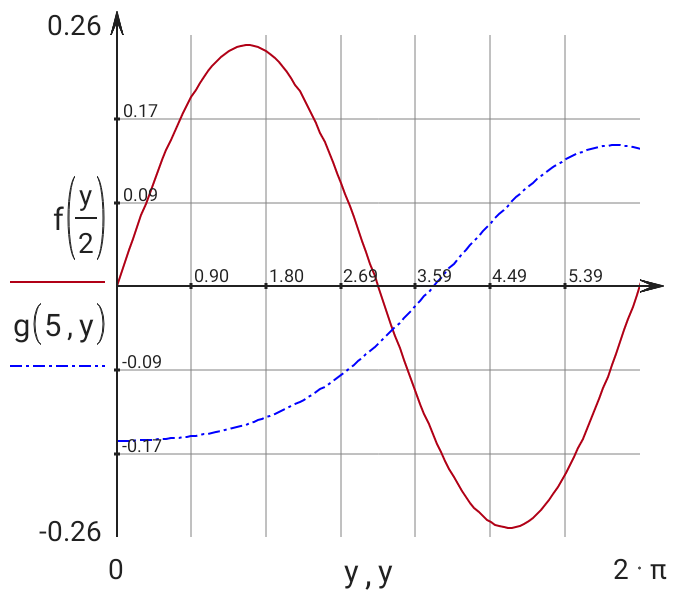
\includegraphics[resolution=320]{graphics/how_to_use_fig9.png} \end{tabular}\end{center}

Para mais detalhes veja exemplos de
''Desenho de função'' e ''Desenho de
Função Polar'' da gaveta de navegação
do app.

\subsection{Desenho Tridimensional}

O desenho 3D exibe um gráfico de uma
função única que depende de dois
argumentos. Para criar tal desenho,
use o botão ''Novo elemento'' na barra
de açõesou o botão ''Adicionar desenho
3D'' da barra de ferramentas:
\begin{center}\begin{tabular}{c} 
\includegraphics[resolution=320]{graphics/how_to_use_fig10.png} \end{tabular}\end{center}
\begin{center}\begin{tabular}{cc}
  $x := \left[ -10,\, -9.5 \,..\, 10 \right]$ &
  $y := \left[ -10,\, -9.5 \,..\, 10 \right]$ \cr
\end{tabular}\end{center}
\begin{center}\begin{tabular}{c} 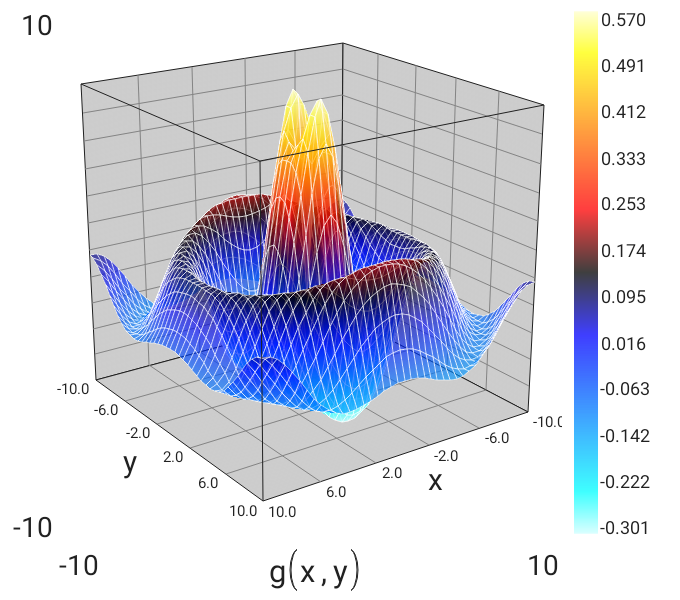
\includegraphics[resolution=320]{graphics/how_to_use_fig11.png} \end{tabular}\end{center}

In the center-bottom field, put the
function name or an equation that
contains exactly two previously
defined intervals. The use of an array
is also possible:
\begin{center}\begin{tabular}{c} 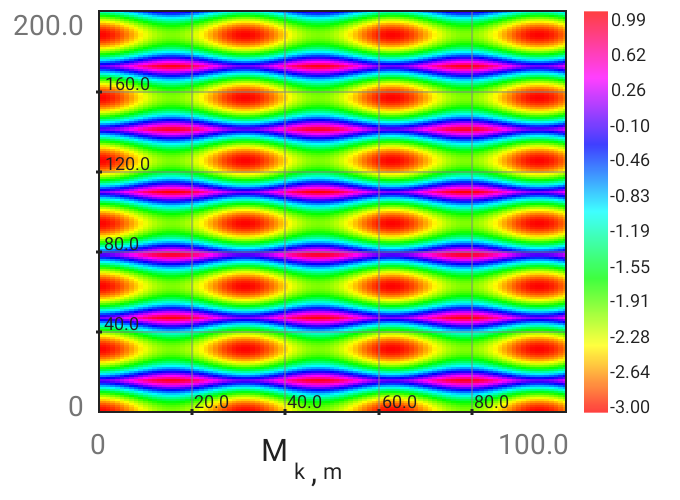
\includegraphics[resolution=320]{graphics/how_to_use_fig12.png} \end{tabular}\end{center}

Para mais detalhes veja o exemplo
''Desenho 3D'' da gaveta de navegação do
app.

\subsection{Text Fragment}

O fragmento de texto exibe texto
simples como este. Para adicionar um
fragmento de texto, use o botão ''Novo
elemento'' na barra de ações ou o botão
''Adicionar fragmento de texto'' da
barra de ferramentas:
\begin{center}\begin{tabular}{c} 
\includegraphics[resolution=320]{graphics/how_to_use_fig13.png} \end{tabular}\end{center}

Se todo o texto dentro de um fragmento
está selecionado usando o menu de
contexto ''Selecionar tudp'', um botão
flutuante ''Propriedades do objeto''
aparece na parte inferior-esquerda da
tela.

Se você tocar neste botão. a janela
''Propriedades do Texto'' será exibida,
onde você pode selecionar a aparência
do texto e ativar a numeração. Por
exemplo, os títulos neste documento
tem a aparência ''Subsection'' com a
numeração ativada.

\subsection{Image}

Você também pode inserir uma imagem de
um arquivo de imagem. Para fazer isso,
use o botão ''Novo elemento'' da barra
de ações ou o botão ''Adicionar arquivo
de imagem'' da barra de ferramentas:
\begin{center}\begin{tabular}{c} 
\includegraphics[resolution=320]{graphics/how_to_use_fig14.png} \end{tabular}\end{center}

A janela de ''Configurações da imagem''
irá aparecer. Nela você pode
selecionar um arquivo com a imagem a
ser inserida e definir o tamanho
necessário da imagem.

Os formatos de imagem a seguir são
suportados: png, bmp, gif, jpeg, svg.

Se você ativar a ''Imagem embutida'' na
janela de ''Configurações de imagem'',
então a imagem será anexada
diretamente no seu documento. Imagem
anexada resulta em um documento único,
mas maior.

Se a ''Imagem embutida'' não estiver
marcada, o arquivo de imagem será
apenas referenciado do que anexado,
i.é. seu documento referencia o
arquivo de imagem fora do documento.
Se você quiser mover seu documento por
favor não esqueça de mover o arquivo
de imagem também.

Você pode alterar as propriedades de
uma imagem já existente. Segure na
área da imagem até que apareça o botão
flutuante ''Propriedades do objeto''. Se
você pressionar este botão, uma janela
com as propriedades da imagem será
exibida.

\section{Ejemplo: Gráfica de una función}
% This is auto-generated file: do not edit!
% Exported from microMathematics Plus, version 2.19.0


Este exemplo demonstra como preparar e
ajustar uma representação gráfica de
uma função. Por exemplo, queremos
desenhar tês funções diferentes:
\begin{center}\begin{tabular}{c}
  $f(x) := 25 + 10 \cdot sin \left( \sqrt{ \left| x \right| } \right) $
\end{tabular}\end{center}
\begin{center}\begin{tabular}{c}
  $g(x) := \frac{2}{{e}^{ \left| x \right|  / 15}} \cdot f \left( x \cdot 50\right) $
\end{tabular}\end{center}
\begin{center}\begin{tabular}{c}
  $h(x) := min \left( f \left( x\right) ,\, g \left( x\right) \right) $
\end{tabular}\end{center}

O argumento da função que representa os
valores-x serão tomados para N pontos
no intervalo [x1, x2]:
\begin{center}\begin{tabular}{ccc}
  $N := 300$ &
  $x1 := -30$ &
  $x2 := 30$ \cr
\end{tabular}\end{center}
\begin{center}\begin{tabular}{c}
  $x := \left[ x1,\, x1 + \left( x2 - x1 \right) / N \,..\, x2 \right]$
\end{tabular}\end{center}

Após as funções e seus argumentos forem
definidos, você pode adicionar a caixa
para desenhar usando o botão ''Novo
elemento'' na barra de ações ou o botão
''Adicionar desenho de função'' a partir
da barra de ferramentas:
\begin{center}\begin{tabular}{c} 
\includegraphics[width=0.45\textwidth]{graphics/function_plot_fig1.png} \end{tabular}\end{center}
\begin{center}\begin{tabular}{c} 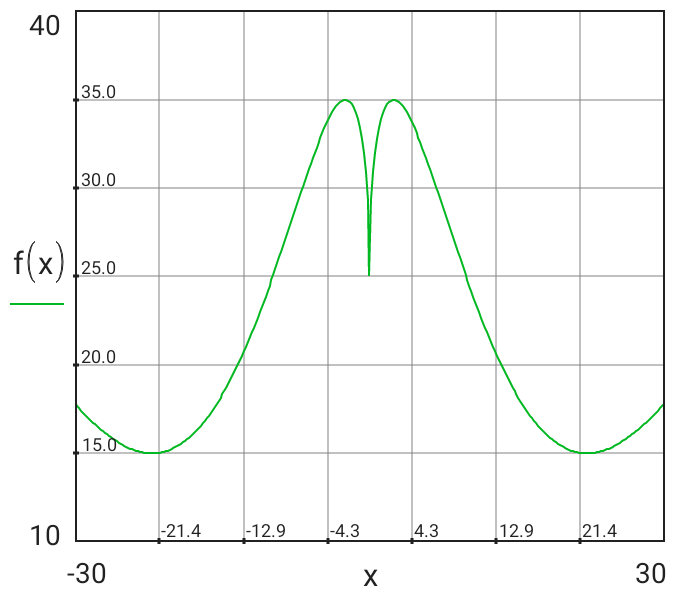
\includegraphics[width=0.45\textwidth]{graphics/function_plot_fig2.png} \end{tabular}\end{center}

A função a ser desenhada será posta no
campo central-esquerdo. Também pode
ser uma função embutida ou declarada
previamente como uma expressão
matemática que contém qualquer outros
operadores e funções.

A função entrada, que representa os
valores-x que serão postos no campo
central-esquerdo. Pode ser uma
variável do tipo intervalo ou uma
expressão matemática que contém uma
variável de intervalo.

Os outros quatro campos descrevem os
limites do desenho. Se estes elementos
premanecerem vazios, o programa
calculará valores correspondentes
automaticamente. Entretanto, você pode
editar estes campos a qualquer momento
e colocar lá os valores que sedejar.

Você pode desenhar diversas funções na
mesma visualização. Para adicionar uma
outra função, selecione a função
(segurando no campo central-esquerdo)
depois qual outra função deve ser
adicionada e toque no botão ''Adicionar
novo argumento'' a partir da barra de
tarefas:
\begin{center}\begin{tabular}{c} 
\includegraphics[width=0.45\textwidth]{graphics/function_plot_fig3.png} \end{tabular}\end{center}
\begin{center}\begin{tabular}{c} 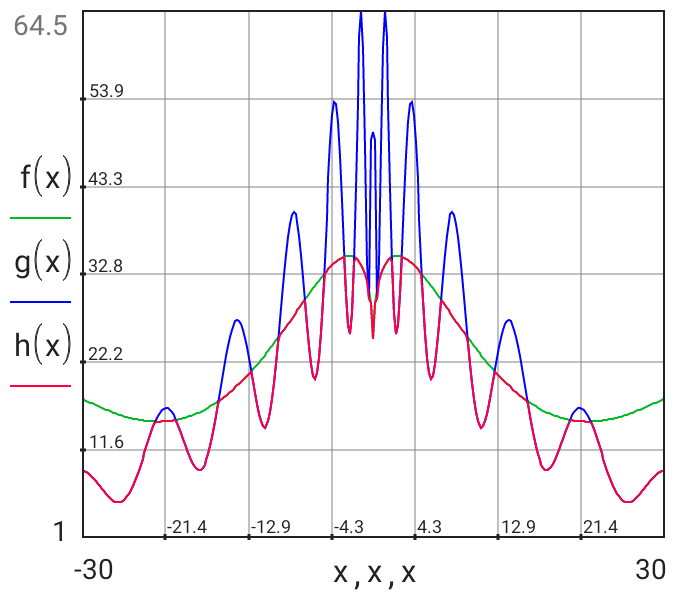
\includegraphics[width=0.45\textwidth]{graphics/function_plot_fig4.png} \end{tabular}\end{center}

Segurando no centro da área de desenho,
o menu de contexto e o botão flutuante
''Propriedades do objeto'' aparecerá.
\begin{center}\begin{tabular}{c} 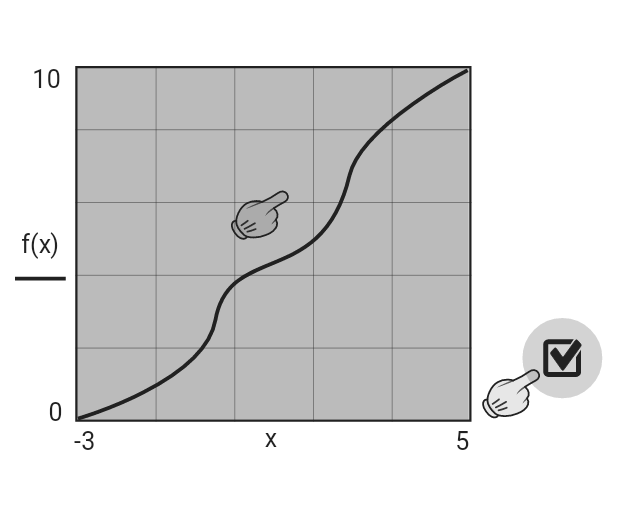
\includegraphics[width=0.45\textwidth]{graphics/function_plot_fig5.png} \end{tabular}\end{center}

Se você tocar no botão flutuante, a
janela de ''Configurações de traço''
será exibida. Aqui, você pode alterar
o tamanho e aparência da área de
desenho. Por exemplo, o gráfico
cruzado parece assim:
\begin{center}\begin{tabular}{c} 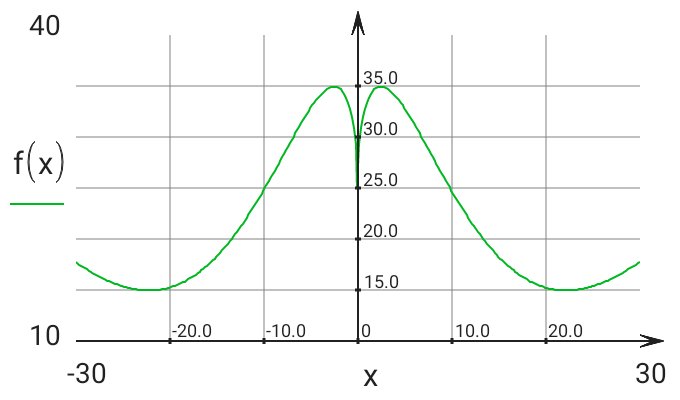
\includegraphics[width=0.45\textwidth]{graphics/function_plot_fig6.png} \end{tabular}\end{center}

Você também pode alterar a cor da linha
de desenho, largura e aparência na
janela ''Configurações da linha''. Ela
aparece ao segurar no marcador de
linha abaixo do nome da função na área
esquerda do desenho:
\begin{center}\begin{tabular}{c} 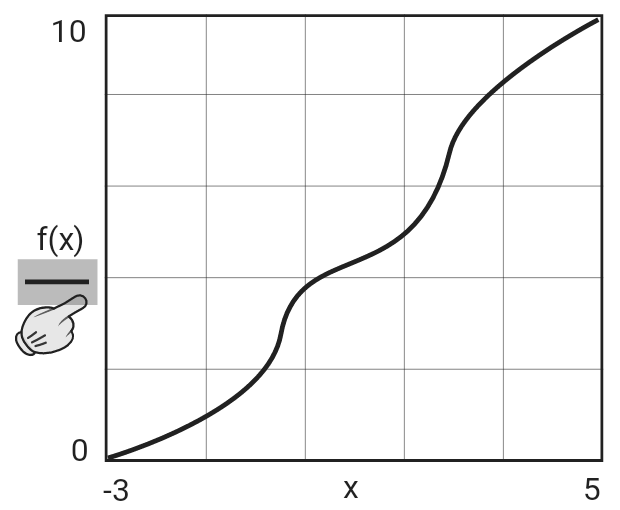
\includegraphics[width=0.45\textwidth]{graphics/function_plot_fig7.png} \end{tabular}\end{center}

For example, we can use dotted lines:
\begin{center}\begin{tabular}{c} 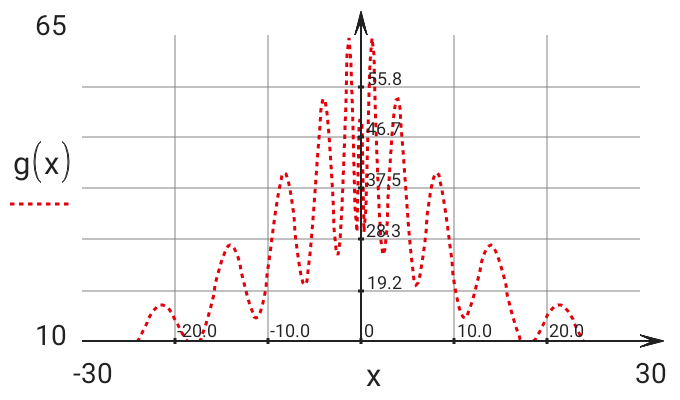
\includegraphics[width=0.45\textwidth]{graphics/function_plot_fig8.png} \end{tabular}\end{center}

O número de eixos e rótulos e cor das
linahs de grade podem ser alteradas na
janela ''Configurações de grade''. Ela
aparece segurando na área livre entre
o valor mínimo de x (-30) e o símbolo
de argumento (x) ou entre o símbolo x
e o valor máximo de x (30) abaixo da
área de desenho:
\begin{center}\begin{tabular}{c} 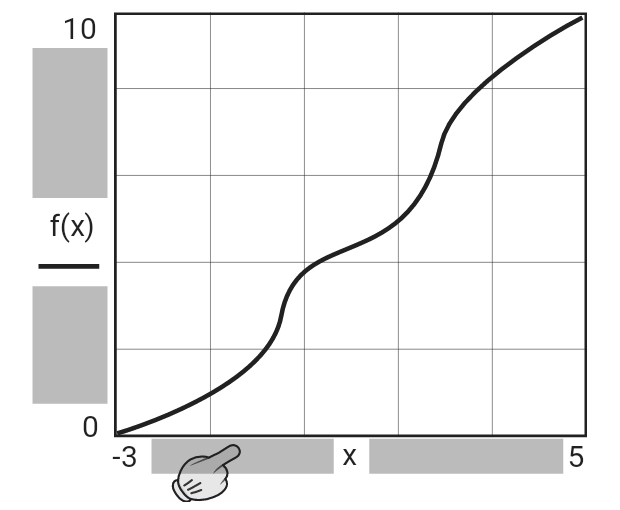
\includegraphics[width=0.45\textwidth]{graphics/function_plot_fig9.png} \end{tabular}\end{center}
\begin{center}\begin{tabular}{c} 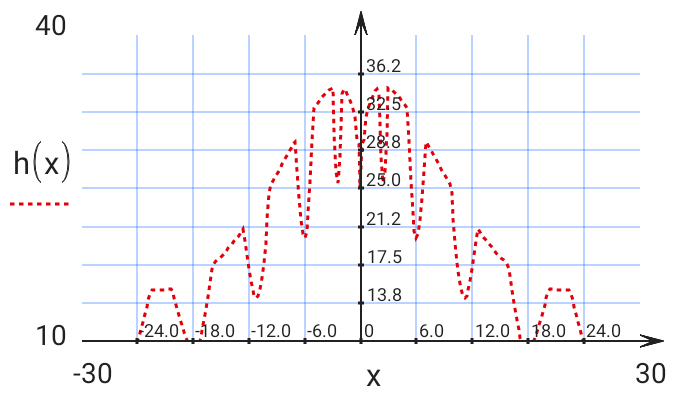
\includegraphics[width=0.45\textwidth]{graphics/function_plot_fig10.png} \end{tabular}\end{center}

Para esconder a grade completamente
apenas defina o número de linhas da
grade para zero nos eixos vertical e
horizontal.

\section{Ejemplo: Gráfica de una función polar}
% This is auto-generated file: do not edit!
% Exported from microMathematics Plus, version 2.18.0


Agora desenharemos várias funções dadas
no sistema de coordenadas polares.
Cada ponto neste sistema é determinado
por uma distância r da origem e o
ângulo f do eixo x.
\begin{center}\begin{tabular}{c} 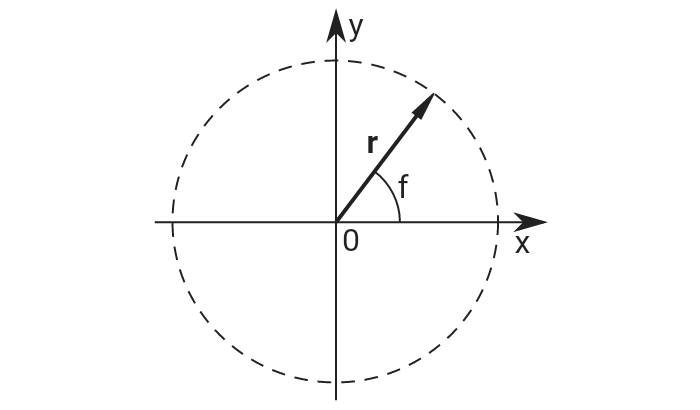
\includegraphics[resolution=320]{graphics/polar_plot_fig1.png} \end{tabular}\end{center}

O ângulo f é nossa variável
independente que muda como está a
seguir:
\begin{center}\begin{tabular}{c}
  $f := \left[ 0.01,\, 0.05 \,..\, 300 \right]$
\end{tabular}\end{center}

A distância r(f) é a nossa variável
dependente. Tendo um par de f e r, nós
podemos tranformar em coordenadas
Cartesianas x e y usando as funções
seno e cosseno:
\begin{center}\begin{tabular}{cc}
  $x(r) := r \cdot cos \left( f\right) $ &
  $y(r) := r \cdot sin \left( f\right) $ \cr
\end{tabular}\end{center}

\subsection{Um caracol}

Definiremos nossa funcção polar em três
passos. A primeira expressão define
uma ''roda'':
\begin{center}\begin{tabular}{ccc}
  $A := 1.1$ &
  $B := 1.271$ &
  $q := 2$ \cr
\end{tabular}\end{center}
\begin{center}\begin{tabular}{c}
  $r1(f) := A + 2 \cdot {sin \left( B \cdot f\right) }^{q}$
\end{tabular}\end{center}

Para desenhar esta função, adicionamos
e caixa de desenho usando o boão ''Novo
elemento'' na barra de ações ou o botão
''Adicionar desenho de função'' a partir
da barra de ferramentas:
\begin{center}\begin{tabular}{c} 
\includegraphics[resolution=320]{graphics/polar_plot_fig2.png} \end{tabular}\end{center}

Ao invés de f e r, usamos aqui regras
previamente definidas para
transformação x e y, onde r1(f) é
usado como um argumento simbólicopara
estas regras:
\begin{center}\begin{tabular}{c} 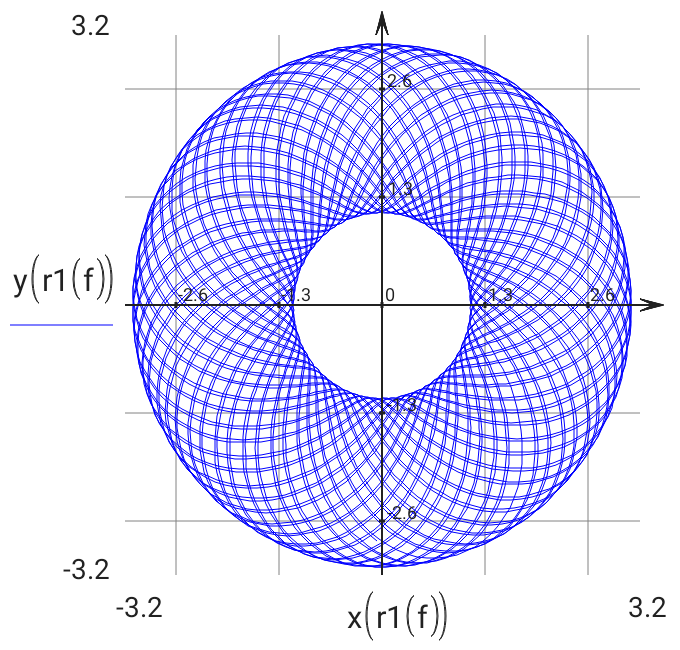
\includegraphics[resolution=320]{graphics/polar_plot_fig3.png} \end{tabular}\end{center}

Então, podemos alterar esta roda como
segue:
\begin{center}\begin{tabular}{c}
  $r2(f) := A + 2 \cdot {sin \left( B \cdot f + 1 \cdot r1 \left( f\right) \right) }^{q}$
\end{tabular}\end{center}
\begin{center}\begin{tabular}{c} 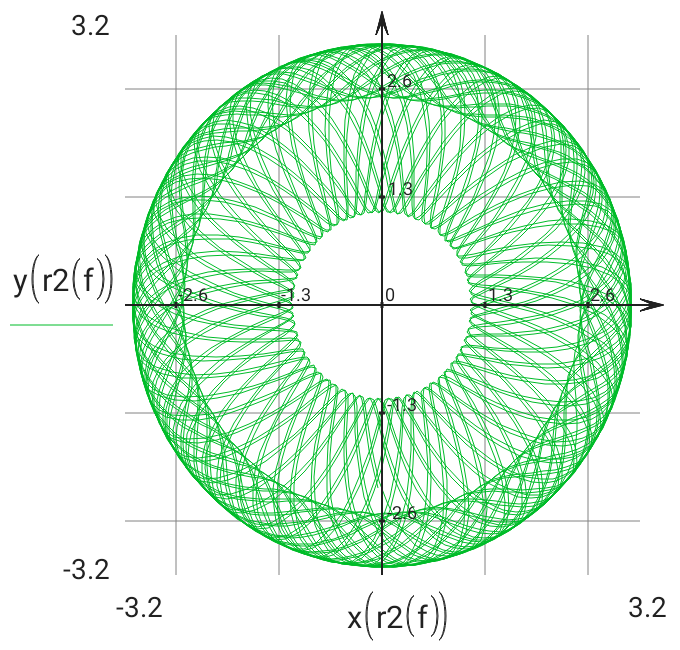
\includegraphics[resolution=320]{graphics/polar_plot_fig4.png} \end{tabular}\end{center}

Finalmente, fazemos a escala da última
função r2(f) usando uma conversão de
inteiro para flutuante que parece uma
função em escada. Como resultado,
obtemos um belo caracol:
\begin{center}\begin{tabular}{c}
  $r(f) := r2 \left( f\right)  \cdot floor \left( f\right)  / 10$
\end{tabular}\end{center}
\begin{center}\begin{tabular}{c} 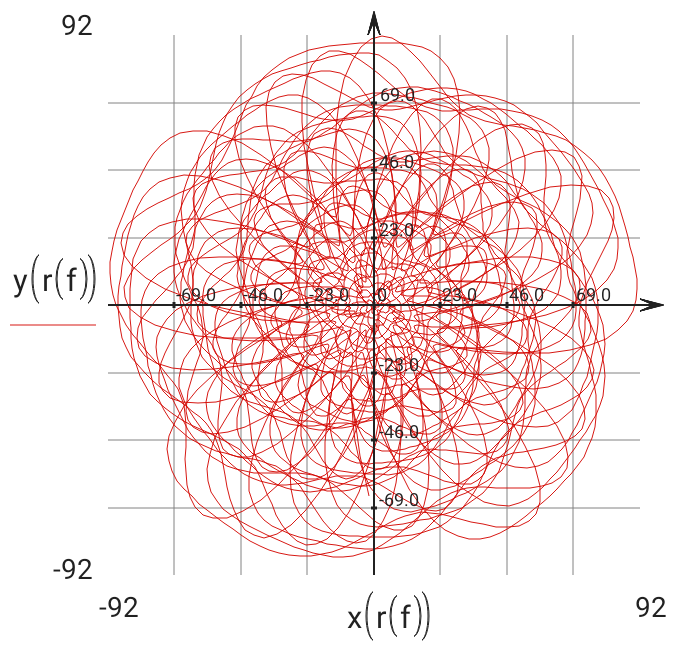
\includegraphics[resolution=320]{graphics/polar_plot_fig5.png} \end{tabular}\end{center}

\subsection{Japanese Maple}

O Maple japonês é muito conhecido pela
forma e cores atraentes de suas
folhas. Estas folhas podem ser
descritas matematicamente e desenhadas
como uma curva no sistema de
coordenadas polares:
\begin{center}\begin{tabular}{c}
  $f := \left[ 0.01,\, 0.02 \,..\, 100 \right]$
\end{tabular}\end{center}
\begin{center}\begin{tabular}{cc}
  $x(r) := r \cdot cos \left( f\right) $ &
  $y(r) := r \cdot sin \left( f\right) $ \cr
\end{tabular}\end{center}
\begin{center}\begin{tabular}{c}
  $s1(f) := \left( 1 + sin \left( f\right)  \right) \cdot \left( 1 - 0.9 \cdot  \left| sin \left( 4 \cdot f\right)  \right|  \right)$
\end{tabular}\end{center}
\begin{center}\begin{tabular}{c}
  $s2(f) := 0.9 + 0.05 \cdot cos \left( 200 \cdot f\right) $
\end{tabular}\end{center}
\begin{center}\begin{tabular}{c}
  $r(f) := floor \left( f\right)  \cdot s1 \left( f\right)  \cdot s2 \left( f\right)  + random \left( 2\right)  - 1$
\end{tabular}\end{center}
\begin{center}\begin{tabular}{c} 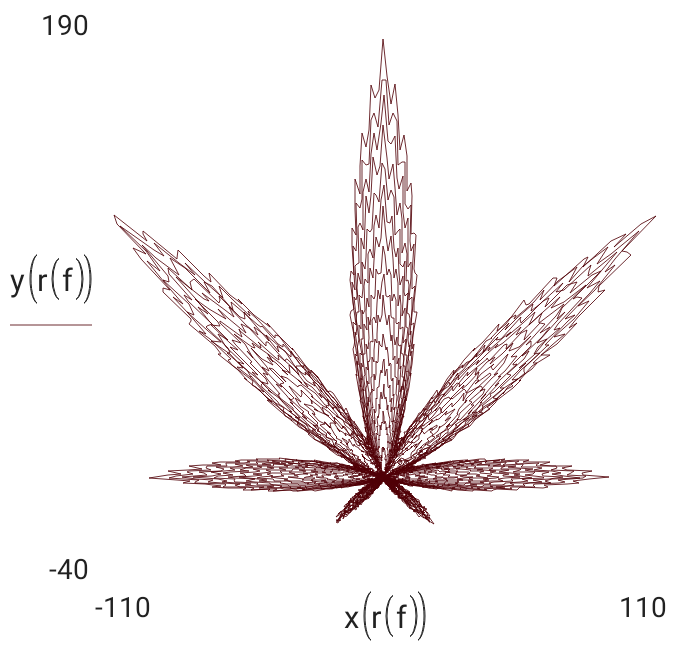
\includegraphics[resolution=320]{graphics/polar_plot_fig6.png} \end{tabular}\end{center}

http://en.wikipedia.org/wiki/Acer\_palmatum

\section{Ejemplo: Gráfico 3D}
% This is auto-generated file: do not edit!
% Exported from microMathematics Plus, version 2.22.0


Este exemplo demonstra desenhos 3D para
três funções diferentes de duas
variáveis.

Primeiro, definimos intervalos para os
argumentos x e y. O intervalo para o
eixo x depende do número de pontos
juntamente com os valores mínimo e
máximo do eixo x, x1 e x2:
\begin{center}\begin{tabular}{ccc}
  $N := 300$ &
  $x1 := -2$ &
  $x2 := 2$ \cr
\end{tabular}\end{center}
\begin{center}\begin{tabular}{c}
  $x := \left[ x1,\, x1 +  \left| x2 - x1 \right|  / N \,..\, x2 \right]$
\end{tabular}\end{center}

O intervalo para o eixo y é definido
analogamente:
\begin{center}\begin{tabular}{ccc}
  $M := 300$ &
  $y1 := -3$ &
  $y2 := 3$ \cr
\end{tabular}\end{center}
\begin{center}\begin{tabular}{c}
  $y := \left[ y1,\, y1 +  \left| y2 - y1 \right|  / M \,..\, y2 \right]$
\end{tabular}\end{center}

Por exemplo, deixe-nos desenhar uma
função trigonométrica que é um produto
de seno e cosseno:
\begin{center}\begin{tabular}{c}
  $F(x,y) := sin \left( 3 \cdot {x}^{2}\right)  \cdot cos \left( {y}^{2}\right) $
\end{tabular}\end{center}

Para criar uma visualização 3D, toque
no botão ''Novo elemento'' da barra de
ações ou pelo botão ''Adicionar desenho
3D'' da barra de ferramentas:
\begin{center}\begin{tabular}{c} 
\includegraphics[width=0.45\textwidth]{graphics/three_d_plot_fig1.png} \end{tabular}\end{center}

Coloque o nome da função F(x,y) no
campo central-inferior:
\begin{center}\begin{tabular}{c} 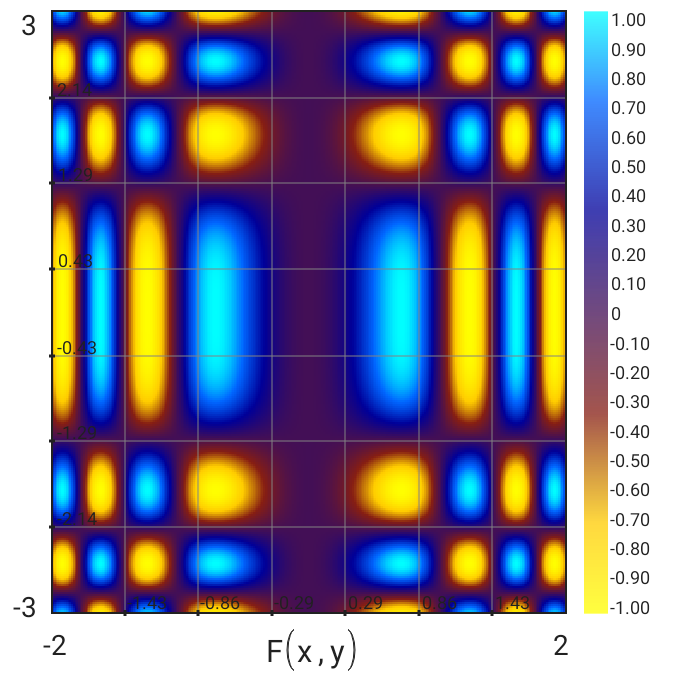
\includegraphics[width=0.45\textwidth]{graphics/three_d_plot_fig2.png} \end{tabular}\end{center}

Os limites do desenho, tamanho do
traçado e aparência, rótulos e grade
podem ser ajustados por analogia com a
função de desenho usando a janela de
configurações do desenho (veja o
exemplo ''Desenhar Função'' da gaveta de
aplicações do app para mais detalhes).
Para abrir esta janela, toque na área
de desenho até que o botão flutuante
''Propriedades do objeto'' apareça, e
então toque neste botão.

Adicionalmente, você pode alterar o
número de rótulos no eixo z e escolher
a paleta de cores na janela
''Configurações do Mapa de Cores''. Esta
janela aparece tocando demoradamente
na barra do eixo z à direita da área
principal do gráfico.
\begin{center}\begin{tabular}{c}
  $R(x,y) := sin \left( 5 \cdot {x}^{2} \cdot \left( y - x \right)\right) $
\end{tabular}\end{center}
\begin{center}\begin{tabular}{c} 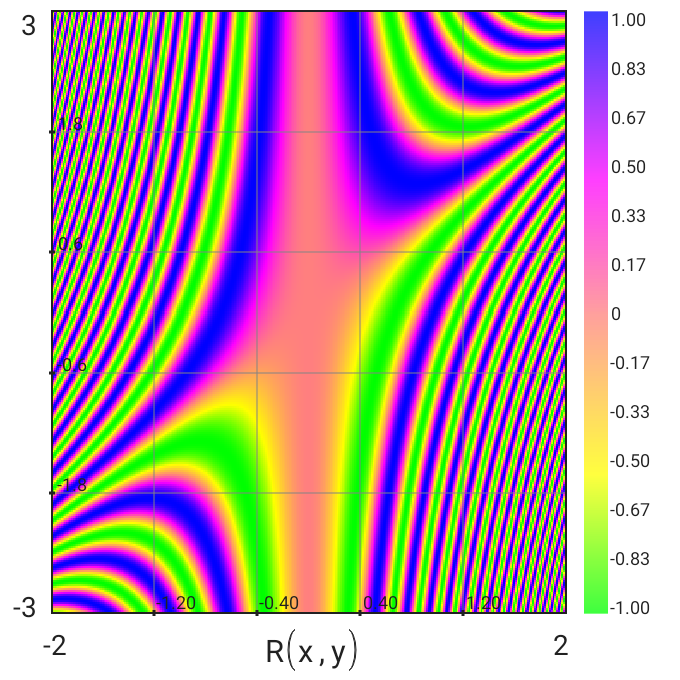
\includegraphics[width=0.45\textwidth]{graphics/three_d_plot_fig3.png} \end{tabular}\end{center}

Uma função de dois argumentos também
pode ser desenhada como uma superfície
no espaço 3D. Este modo pode ser
ativado na janela de ''Configurações de
Desenho'' que aparece se você tocar no
botão flutuante ''Propridades do
objeto'' após tocar demoradamente na
área de desenho. Deixe-nos desenhar a
seguinte função, usando conjuntos para
poder diminuir o tempo de cálculo:
\begin{center}\begin{tabular}{cccc}
  $N := 100$ &
  $n := \left[ 0,\, 1 \,..\, N \right]$ &
  $x1 := -15$ &
  $x2 := 15$ \cr
\end{tabular}\end{center}
\begin{center}\begin{tabular}{cccc}
  $M := 100$ &
  $m := \left[ 0,\, 1 \,..\, M \right]$ &
  $y1 := -15$ &
  $y2 := 15$ \cr
\end{tabular}\end{center}
\begin{center}\begin{tabular}{c}
  $x_{n}  := {\left( x1 +  \left( x2 - x1\right)  \cdot n / N \right)}^{2}$
\end{tabular}\end{center}
\begin{center}\begin{tabular}{c}
  $y_{m}  := {\left( y1 +  \left( y2 - y1\right)  \cdot m / M \right)}^{2}$
\end{tabular}\end{center}
\begin{center}\begin{tabular}{c}
  $r_{n,\, m}  := 0.04 \cdot x_{n}  + 0.02 \cdot y_{m} $
\end{tabular}\end{center}
\begin{center}\begin{tabular}{c}
  $t_{n,\, m}  := \left( x_{n}  + 0.05 \cdot y_{m}  \right) \cdot exp \left( 1 - r_{n,\, m} \right) $
\end{tabular}\end{center}
\begin{center}\begin{tabular}{c}
  $F_{n,\, m}  := \frac{sin \left( x_{n}  + 0.1 \cdot y_{m} \right) }{0.15 + r_{n,\, m} } + \frac{t_{n,\, m} }{10}$
\end{tabular}\end{center}
\begin{center}\begin{tabular}{c} 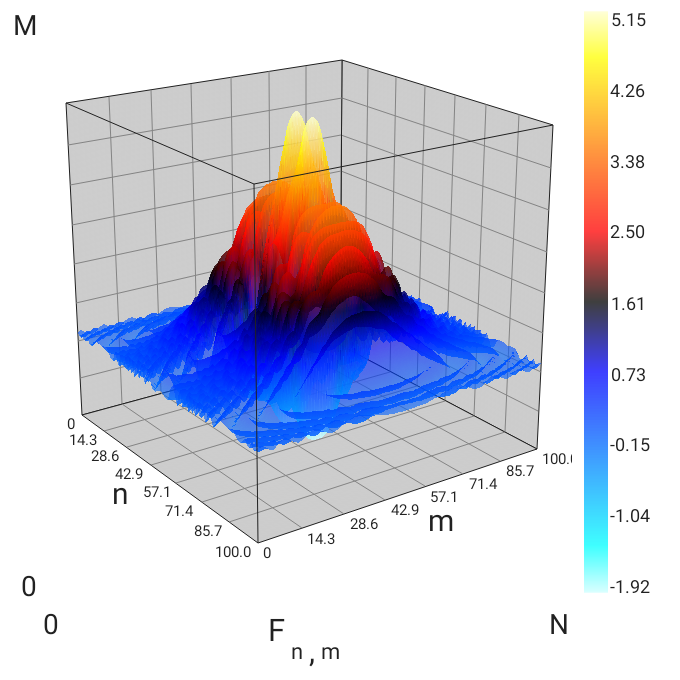
\includegraphics[width=0.45\textwidth]{graphics/three_d_plot_fig4.png} \end{tabular}\end{center}

Para o desenho de superfícies, existem
configurações adicionais mostradas na
janela de ''Configurações de Desenho''.
Você pode escolher se deseja que as
linhas da malha devem ser mostradas.
Selecione a opacidade para a cor da
malha, defina os ângulo de rotação e a
elevação da caixa de desenho. Por
exemplo, a superfície desenhada
anteriormente com outros ângulos de
rotação e elevação se parece com: 
\begin{center}\begin{tabular}{c} 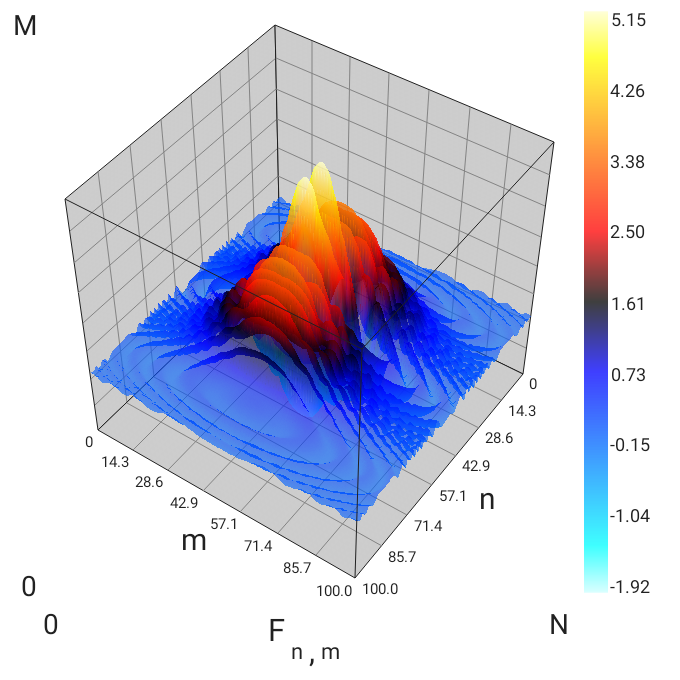
\includegraphics[width=0.45\textwidth]{graphics/three_d_plot_fig5.png} \end{tabular}\end{center}

\section{Ejemplo: Series e integrales}
% This is auto-generated file: do not edit!
% Exported from microMathematics Plus, version 2.17.4


Esse exemplo demonstra como calcular
séries e integrais.

\subsection{Taylor series}

Na matemática, séries de Taylor são uma
representação de uma função como uma
soma infinita de termos que são
calculados a partir da derivada dos
valores da função num único ponto.

Por exemplo, Ts(x,N) é a expansão de
Taylor de uma função com argumento x e
N número de termos:
\begin{center}\begin{tabular}{c}
  $Ts(x,N) := \displaystyle\sum_{n=0}^{N} \frac{{ \left( -1\right) }^{n}}{\left( 2 \cdot n \right)! } \cdot {x}^{2 \cdot n}$
\end{tabular}\end{center}

Esta expansão se aproxima da função
cosseno:
\begin{center}\begin{tabular}{c}
  $s(x) := cos \left( x\right) $
\end{tabular}\end{center}

Se desenharmos as duas funções juntas
para o mesmo intervalo, elas parecem
iguais:
\begin{center}\begin{tabular}{c}
  $x := \left[ 0,\, 0.1 \,..\, 2 \cdot {\pi} \right]$
\end{tabular}\end{center}
\begin{center}\begin{tabular}{c} 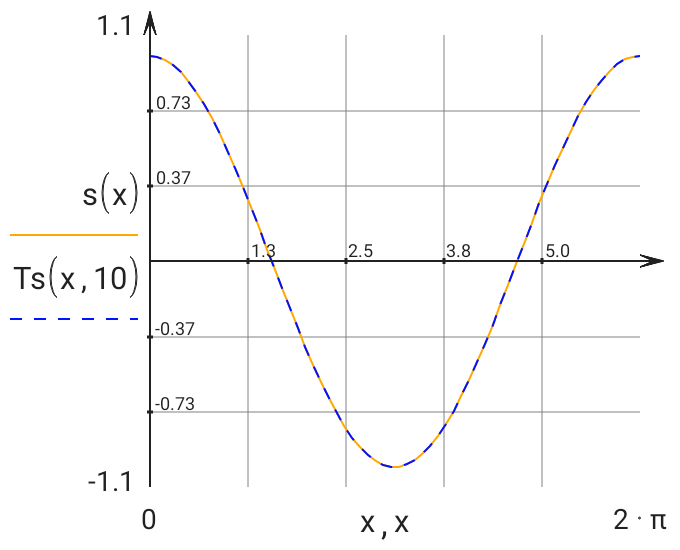
\includegraphics[resolution=320]{graphics/series_and_integrals_fig1.png} \end{tabular}\end{center}

Entretando, há um erro numérico devido
ao número limitado de termos de
aproximação N. A função a seguir
$\Delta$(x,N) descreve este erro:
\begin{center}\begin{tabular}{c}
  ${\Delta}(x,N) :=  \left| s \left( x\right)  - Ts \left( x,\, N\right)  \right| $
\end{tabular}\end{center}

Podemos desenhar esta função em
coordenadas logarítmicas e ver que o
erro numérico diminuirá se tivermos
mais termos na soma de Taylor:
\begin{center}\begin{tabular}{c}
  $N := \left[ 3,\, 4 \,..\, 13 \right]$
\end{tabular}\end{center}
\begin{center}\begin{tabular}{c} 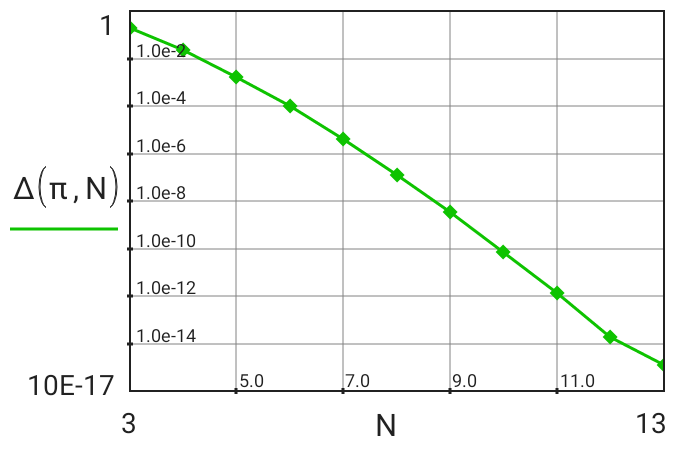
\includegraphics[resolution=320]{graphics/series_and_integrals_fig2.png} \end{tabular}\end{center}

\subsection{Série Binomial}

Consideremos esta função potência:
\begin{center}\begin{tabular}{c}
  $f(x,{\alpha}) := {\left( 1 + x \right)}^{{\alpha}}$
\end{tabular}\end{center}

Esta função pode ser aproximada usando
Série Binomial:
\begin{center}\begin{tabular}{c}
  $Tf(x,{\alpha},N) := \displaystyle\sum_{n=0}^{N}  \left( \displaystyle\prod_{k=1}^{n} \frac{{\alpha} - k + 1}{k}\right)  \cdot {x}^{n}$
\end{tabular}\end{center}

Podemos também desenhar as duas funções
(a função de potência dada e sua
aproximação) juntas no mesmo gráfico:
\begin{center}\begin{tabular}{c} 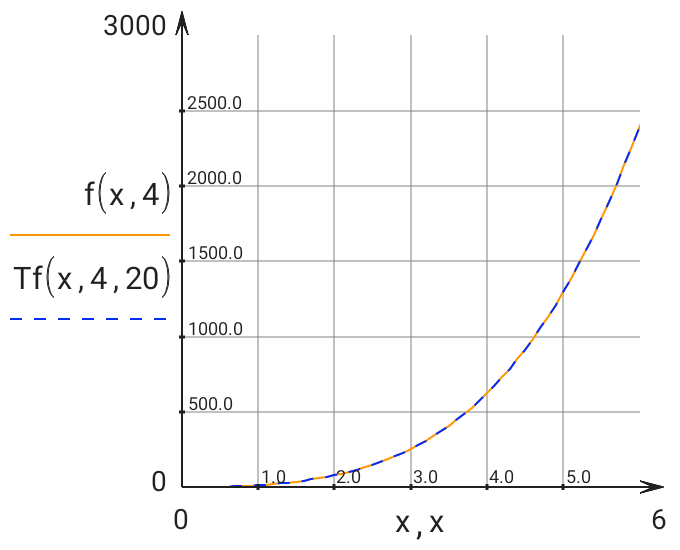
\includegraphics[resolution=320]{graphics/series_and_integrals_fig3.png} \end{tabular}\end{center}

\subsection{Integrais}

Também é possível calcular uma integral
definida numericamente usando o método
de Simpson. Por exemplo, podemos
calcular a integral usando o elemento
''Visualização de resultado'':
\begin{center}\begin{tabular}{c}
  $\displaystyle\int_{0}^{3 \cdot pi / 2}{cos \left( \frac{2 \cdot x}{9}\right) }^{-2}\, dx = 7.79423$
\end{tabular}\end{center}

A solução analítica é
\begin{center}\begin{tabular}{ccc}
  $I := \frac{9 \cdot \sqrt{3} }{2}$ &
  ,    &
  $I = 7.79423$ \cr
\end{tabular}\end{center}

O erro numérico pode ser calculado
como:
\begin{center}\begin{tabular}{c}
  $\displaystyle\int_{0}^{3 \cdot pi / 2}{cos \left( \frac{2 \cdot x}{9}\right) }^{-2}\, dx - I = 4.26681E-9$
\end{tabular}\end{center}

Este erro depende do valor de ''Número
de dígitos significativos no
resultado'' que pode ser alterado na
janela ''Configurações do Documento''
disponível a partir da barra de ações:
\begin{center}\begin{tabular}{c} 
\includegraphics[resolution=320]{graphics/series_and_integrals_fig4.png} \end{tabular}\end{center}

Se este valor aumentou, o limiar que
controla a precisão do método de
Simpson também aumentará.

\section{Sobre microMathematics Plus}
% This is the second part of the file about_micromath.tex
\subsection{Autores}

\begin{enumerate}
\item Mikhail Kulesh,
mikhail.kulesh@gmail.com

\item Caio Roberto Ramos da Silva
(Brazilian Portuguese translation),
caiorrs@gmail.com

\item Yubin Hsu
(Chinese translation),
yubin.taiwan@gmail.com

\item Linsui
(Chinese translation),
linsui555@gmail.com
\end{enumerate}

\subsection{Icono de la app}

El icono de la aplicación se genera a partir de la siguiente
función definida en el
sistema de coordenadas polares:
\begin{center}\begin{tabular}{c}
                $f := \left[ 0.01,\, 0.03 \,..\, 150 \right]$
\end{tabular}\end{center}
\begin{center}\begin{tabular}{c}
                $s(f) := 4 + sin \left( 5 \cdot f\right)  + \frac{sin \left( 10 \cdot f\right) }{2} + \frac{sin \left( 60 \cdot f\right) }{6}$
\end{tabular}\end{center}
\begin{center}\begin{tabular}{c}
                $r(f) := 0.9 \cdot \left( 1 + f / 50 \right) \cdot s \left( f\right) $
\end{tabular}\end{center}
\begin{center}\begin{tabular}{c}
                $x(f) := r \left( f\right)  \cdot cos \left( f\right) $
\end{tabular}\end{center}
\begin{center}\begin{tabular}{c}
                $y(f) := r \left( f\right)  \cdot sin \left( f\right) $
\end{tabular}\end{center}
\begin{center}\begin{tabular}{c} 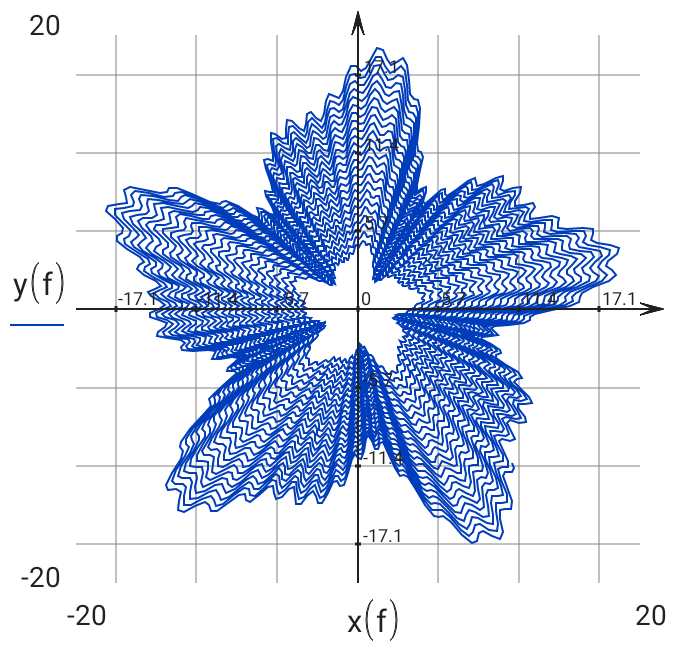
\includegraphics[width=0.45\textwidth]{graphics/about_micromath_fig1.png} \end{tabular}\end{center}

2014-2020, Bremen, Alemania
\end{document}